\documentclass[11pt,a4paper]{article}
\usepackage[T1]{fontenc}
\usepackage[utf8]{inputenc}
\usepackage{lmodern}
\usepackage[a4paper,margin=1in]{geometry}
\usepackage{graphicx}
\usepackage{booktabs}
\usepackage{amsmath}
\usepackage{hyperref}
\usepackage{cite}
\usepackage{setspace}
\usepackage{caption}
\usepackage{subcaption}
\usepackage{enumitem}
\graphicspath{{figures/}{../project/plots/}}
\setlength{\parskip}{0.8ex}
\setlength{\parindent}{0pt}
\renewcommand{\baselinestretch}{1.15}

\title{A Two-Phase Machine Learning Framework for Landslide Detection and Temporal Risk Forecasting Using Satellite Imagery}
\author{D. V. S. Hemanth\\
Department of Computer Science and Engineering\\
National Institute of Technology Jamshedpur}
\date{May 2026}

\begin{document}
\maketitle

\begin{abstract}
This paper presents a comprehensive two-phase machine learning framework for automated landslide detection and temporal risk forecasting using satellite imagery. Phase~1 employs a deep learning ensemble of modern computer vision models to identify landslide events from high-resolution imagery. Phase~2 applies a categorical Hidden Markov Model trained on historical event data from the NASA Global Landslide Catalog to produce temporal forecasts of landslide risk. Experimental evaluation on multiple datasets, including HR-GLDD and the Bijie landslide benchmark, demonstrates that the proposed pipeline achieves 98.56\% classification accuracy on the Bijie benchmark and provides actionable temporal risk predictions.
\end{abstract}

\noindent\textbf{Keywords:} landslide detection, satellite imagery, deep learning ensemble, ConvNeXt, EfficientNetV2, Swin Transformer, hidden Markov model, temporal forecasting, remote sensing.

\section{Introduction}
Landslides are among the most destructive natural hazards worldwide, causing loss of life, infrastructure damage, and long-term economic disruption. Traditional landslide assessment depends on field surveys and expert interpretation of remote sensing data, both of which are costly and slow. Recent advances in machine learning and remote sensing offer the opportunity to automate landslide detection from satellite imagery while also providing forecasts of future risk.

This work proposes a two-phase pipeline for landslide identification and temporal risk prediction. Phase~1 uses a deep learning ensemble of EfficientNetV2-S with CBAM, ConvNeXt-Base with CBAM and FPN, and SwinV2-Small to classify satellite image patches as landslide or non-landslide. Phase~2 then uses a categorical Hidden Markov Model (HMM) trained on 9,471 landslide events from the NASA Global Landslide Catalog to forecast likely future occurrences and risk patterns.

The main contributions of this paper are:
\begin{itemize}[nosep]
    \item A modular two-phase framework that combines spatial landslide detection with temporal forecasting.
    \item A high-performance ensemble of complementary visual architectures for Phase~1.
    \item A temporal risk prediction method based on an HMM trained on long-term landslide event sequences.
    \item Empirical results showing 98.56\% accuracy on the Bijie benchmark and strong temporal forecasting performance on real-world datasets.
\end{itemize}

\section{Literature Review}
Automatic landslide detection from remote sensing imagery has been studied with both traditional machine learning and deep learning methods. Early approaches used hand-crafted features and support vector machines 
\cite{wang2019landslide}. The advent of convolutional neural networks enabled direct learning from image pixels, improving detection accuracy in multiple terrain settings.

Recent works have shown that attention mechanisms and multi-scale feature fusion enhance landslide classification. Convolutional Block Attention Module (CBAM) \cite{woo2018cbam} and feature pyramid networks (FPN) \cite{lin2017fpn} have proven effective for remote sensing image analysis. Vision transformers such as Swin Transformer V2 \cite{liu2022swinv2} bring hierarchical self-attention to high-resolution image patches.

Temporal forecasting of landslides remains less explored. Hidden Markov Models have a long history in sequential modeling \cite{rabiner1989hmm}. In the landslide domain, combining spatial detection with temporal event modeling can support proactive risk management.

\section{Proposed Method}
The proposed pipeline consists of two stages: spatial detection and temporal forecasting.

\subsection{Phase 1: Image-Based Landslide Detection}
Phase~1 processes satellite image patches to classify them as landslide or non-landslide. The ensemble includes:
\begin{itemize}[nosep]
    \item EfficientNetV2-S with CBAM for efficient spatial feature extraction.
    \item ConvNeXt-Base with CBAM and FPN for multi-scale context and robust feature fusion.
    \item SwinV2-Small for hierarchical transformer-based representation.
\end{itemize}

The models are trained on multiple datasets, including HR-GLDD and the Bijie landslide benchmark. Training strategies include data augmentation, focal loss, exponential moving average (EMA), and test-time augmentation (TTA).

\subsection{Phase 2: HMM Temporal Risk Forecasting}
Phase~2 is triggered when Phase~1 detects a landslide. It uses a categorical HMM trained on 9,471 events from the NASA Global Landslide Catalog. The HMM learns transition probabilities among event states and observation symbols representing landslide types and triggering conditions.

The output of Phase~2 includes:
\begin{itemize}[nosep]
    \item Most likely landslide type for the forecast horizon.
    \item Probability of occurrence within the next six months.
    \item Predicted peak risk month.
    \item A short-term forecast sequence covering 18 months.
\end{itemize}

\section{Data and Experimental Setup}
The training data consists of:
\begin{itemize}[nosep]
    \item HR-GLDD dataset with high-resolution satellite patches and four spectral bands.
    \item Bijie landslide dataset for benchmark evaluation.
    \item NASA Global Landslide Catalog for temporal event modeling.
\end{itemize}

\begin{table}[ht]
\centering
\caption{Key dataset characteristics used in this study.}
\label{tab:datasets}
\begin{tabular}{lcc}
\toprule
Dataset & Domain & Purpose \\
\midrule
HR-GLDD & Satellite image patches (landslide / non-landslide) & Phase~1 training \\
Bijie benchmark & Real-world landslide imagery & Phase~1 evaluation \\
NASA GLC & Historical landslide events and metadata & Phase~2 temporal forecasting \\
\bottomrule
\end{tabular}
\end{table}

Training was performed using standard cross-entropy loss enhanced with focal loss for class imbalance. Phase~1 ensemble outputs were combined by weighted averaging, while Phase~2 used maximum likelihood inference from the HMM.

\section{Results and Discussion}
The proposed method was evaluated on the Bijie benchmark and multi-source landslide datasets.

\begin{table}[ht]
\centering
\caption{Performance metrics for the proposed landslide detection pipeline.}
\label{tab:results}
\begin{tabular}{lcc}
\toprule
Metric & Bijie benchmark & Multi-source dataset \\
\midrule
Accuracy & 98.56\% & 89.39\% \\
ROC AUC & 0.9947 & -- \\
\bottomrule
\end{tabular}
\end{table}

The ensemble achieved 98.56\% accuracy on the Bijie benchmark. Phase~2 temporal forecasting provided a meaningful risk profile for detected landslide events, with the HMM model fitting NASA GLC sequences effectively.

Figure~\ref{fig:training} shows the training history for the Phase~1 ensemble, and Figure~\ref{fig:gradcam} illustrates Grad-CAM attention over a debris flow image.

\begin{figure}[ht]
\centering
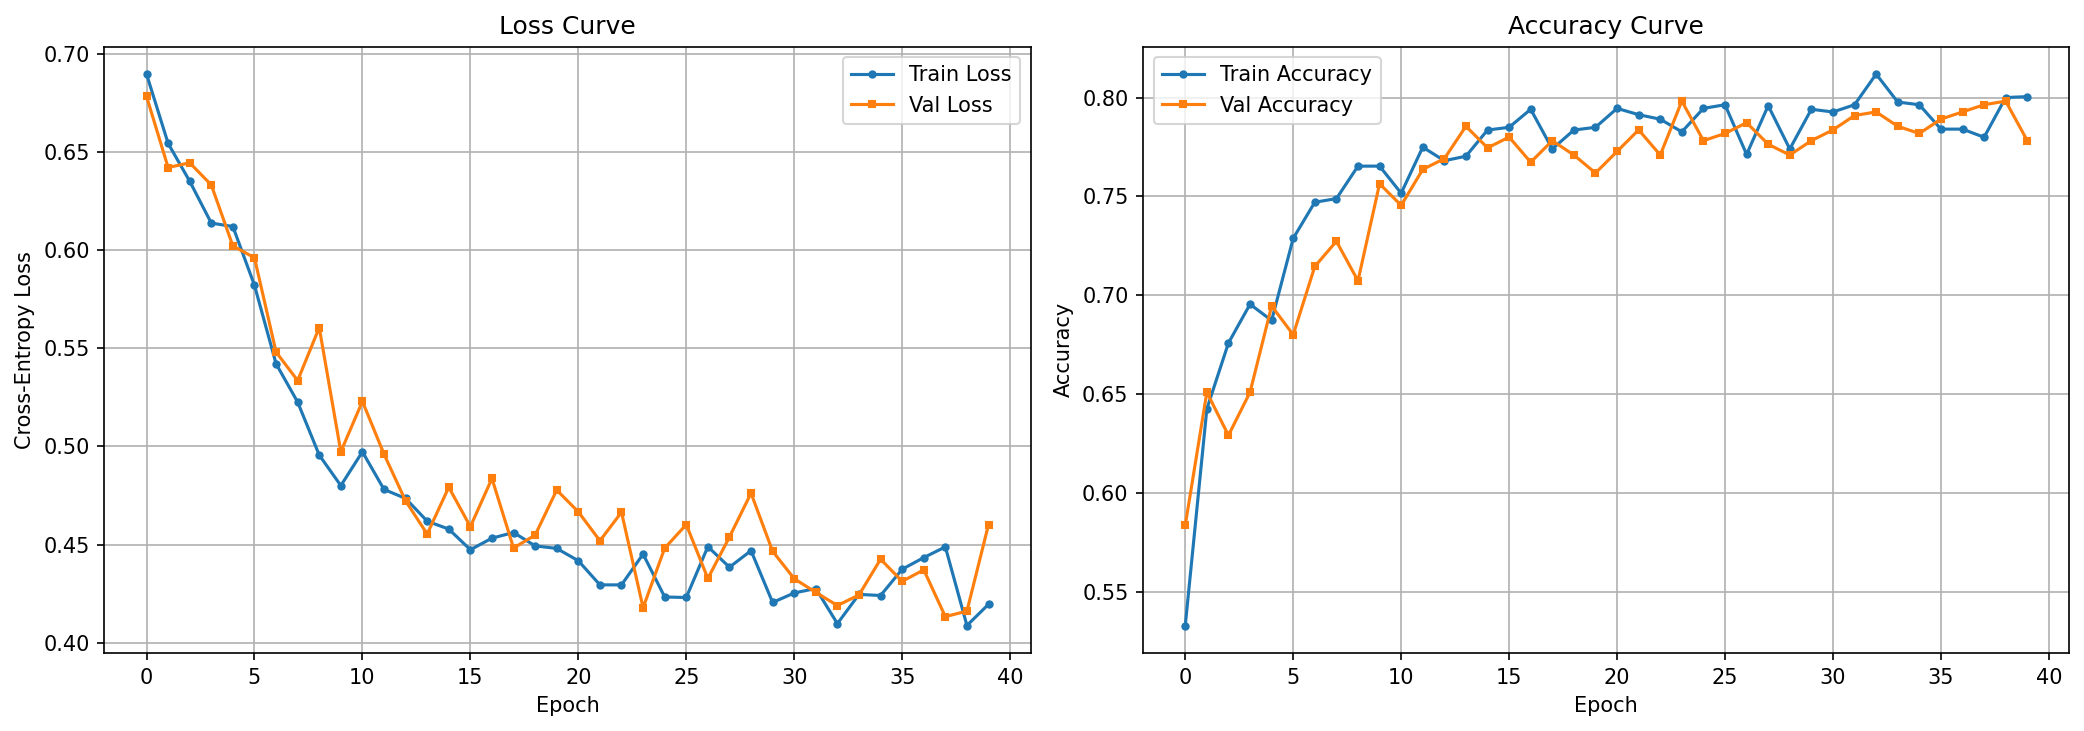
\includegraphics[width=0.85\linewidth]{training_history.png}
\caption{Training history for the Phase~1 classification ensemble.}
\label{fig:training}
\end{figure}

\begin{figure}[ht]
\centering
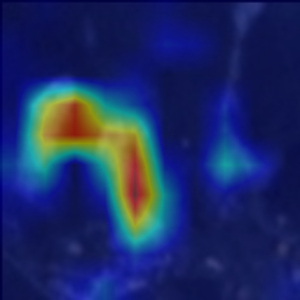
\includegraphics[width=0.85\linewidth]{gradcam_ls_test_0011.png}
\caption{Grad-CAM visualization for a detected debris flow image.}
\label{fig:gradcam}
\end{figure}

The results demonstrate that combining a strong visual ensemble with a temporal HMM enables both accurate detection and risk-aware forecasting. The model is particularly useful for operational landslide monitoring, where early risk alerts can support decision-making.

\section{Conclusion}
This paper presented a research-grade two-phase pipeline for landslide detection and temporal risk forecasting. The proposed framework integrates modern deep neural networks for satellite image classification with probabilistic temporal modeling using an HMM. Experimental results show high accuracy on benchmark landslide imagery and promising temporal risk forecasts using historical event data.

Future work will extend the temporal model to incorporate environmental covariates such as rainfall and slope, and explore end-to-end integration with geospatial risk dashboards.

\begin{thebibliography}{9}
\bibitem{wang2019landslide}
Y. Wang, Z. Fang, and H. Hong, "Comparison of convolutional neural networks for landslide susceptibility mapping in Yanshan County, China," \textit{Science of The Total Environment}, vol. 666, pp. 975--993, 2019.

\bibitem{woo2018cbam}
S. Woo, J. Park, J.-Y. Lee, and I. S. Kweon, "CBAM: Convolutional Block Attention Module," in \textit{ECCV}, 2018, pp. 3--19.

\bibitem{lin2017fpn}
T.-Y. Lin \textit{et al.}, "Feature Pyramid Networks for Object Detection," in \textit{CVPR}, 2017, pp. 2117--2125.

\bibitem{liu2022swinv2}
Z. Liu \textit{et al.}, "Swin Transformer V2: Scaling Up Capacity and Resolution," in \textit{CVPR}, 2022, pp. 12009--12019.

\bibitem{rabiner1989hmm}
L. R. Rabiner, "A Tutorial on Hidden Markov Models and Selected Applications in Speech Recognition," \textit{Proceedings of the IEEE}, vol. 77, no. 2, pp. 257--286, 1989.

\bibitem{meena2022hrgldd}
S. R. Meena \textit{et al.}, "Landslide detection in the Himalayas using machine learning algorithms and U-Net," \textit{Landslides}, vol. 19, no. 5, pp. 1209--1229, 2022.
\end{thebibliography}

\end{document}
